\documentclass[sigconf]{acmart}
\usepackage{graphicx}
\usepackage{natbib}
\usepackage{amsmath}
\usepackage{amssymb}
\usepackage{subcaption}
\usepackage{multicol}
\usepackage{tabulary}
\usepackage[utf8]{inputenc}

% Copyright
\setcopyright{rightsretained}

%Conference
\acmConference[ISFPGA'18]{26th ACM/SIGDA International Symposium on Field-Programmable Gate Arrays}{February 2018}{Monterey, California, USA} 
\acmYear{2018}
\copyrightyear{2017}


\title{Aligning Time-Varying Fields of View Using Feature Detection on FPGA}

\author{Robert Taglang}
\affiliation{%
	\institution{Drexel University}
	\city{Philadelphia} 
	\state{Pennsylvania} 
}
\email{rob@taglang.io}

\author{Prawat Nagvajara Ph.D}
\affiliation{%
	\institution{Drexel University}
	\city{Philadelphia} 
	\state{Pennsylvania} 
}
\email{nagvajara@coe.drexel.edu}

\begin{document}

\begin{abstract}
	This paper presents a system for detecting features using an FPGA implementation of SURF (Speeded-Up Robust Features), and aligning video streams by applying an adaptive transform generated based on key features. As a result the proposed technique can align time-varying field of view sources. The results include an efficient FPGA implementation of SURF and a real-time affine transform for aligning video sources to achieve minimal latency. The design is based on pipelining the SURF computation and using address mapping for fast transformations. The implementation was performed on a ZedBoard Zynq-7000 ARM/FPGA SoC Development board with two 640 by 480 resolution video streams at 30 frames per second. This approach has potential for future applications including stabilization by matching features between consecutive video frames.
\end{abstract}

\maketitle

\section{Introduction}

The fusion of data from two or more sensors has been well-researched \cite{wang_multi-focus_2011} \cite{li_multi-sensor_1994}, though these approaches typically discuss the process of fusing images which have been pre-aligned. Pre-computed transforms used to align the frames of two cameras are not robust to variations. Some approaches have made use of additional hardware sensors in order to correct against these variations \cite{chappell_exploiting_2006}. The approach presented in this thesis seeks to perform this correction in real time, completely in hardware, using feature detection on a Field Programmable Gate Array (FPGA) using the design shown in Figure \ref{fig_block_diagram}.

\begin{figure}[h]
	\centering
	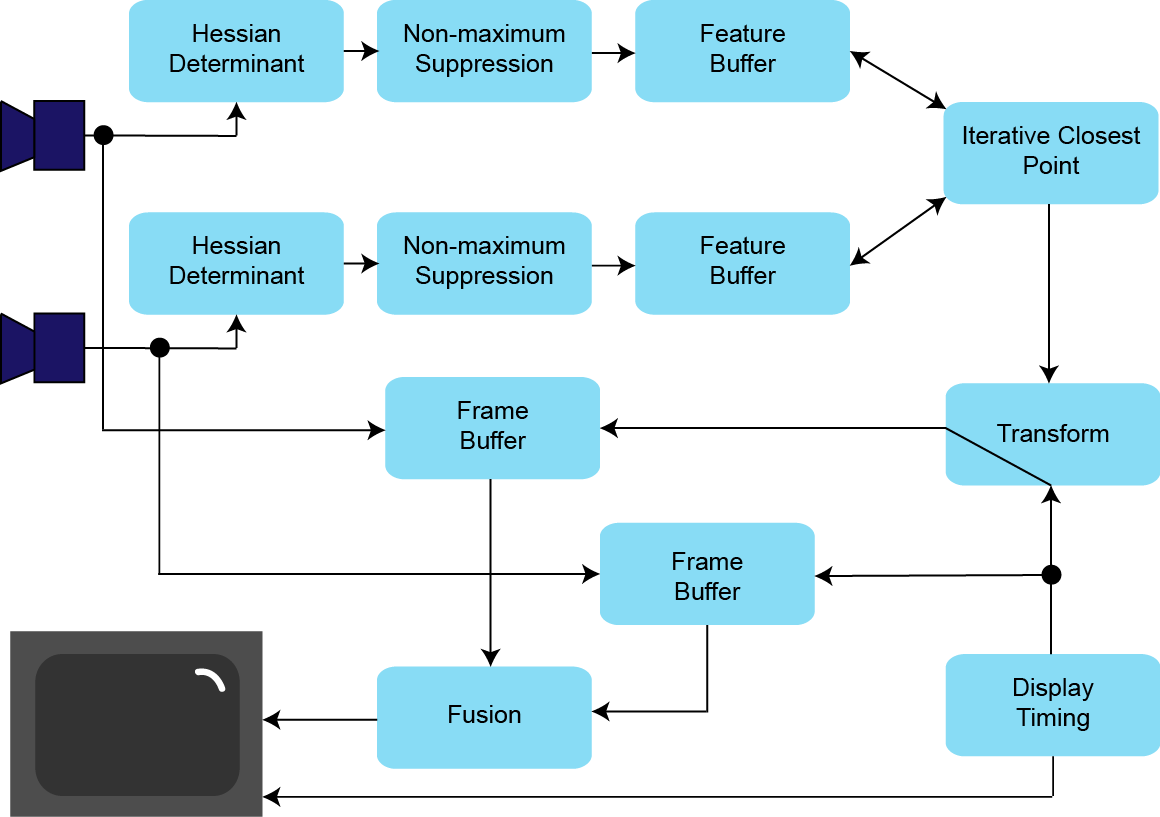
\includegraphics[width=\columnwidth]{figures/block/blockdiagram}
	\caption{Block diagram of the proposed system for alignment and fusion}
	\label{fig_block_diagram}
\end{figure}

In order to align two images, one is treated as the reference image, and the other is the transformed image which needs to be aligned with the reference image. As such the problem can be broken into four major components. 

\begin{enumerate}
	\item Detecting feature points in the two images (Hessian Determinant, Non-maximum Suppression, Feature Buffer block).
	\item Computing the transform which maps the transformed image into the space of the reference image (Iterative Closest Point block).
	\item Applying the computed transform to the transformed image (Transform, Frame Buffer, Display Timing block).
	\item Fusion of the reference and transformed image (Fusion block).
\end{enumerate}

Feature points are detected using some of the techniques from Speeded-up Robust Features (SURF) which makes use of Hessian determinants to detect points of interest in multiple scale spaces. High magnitude features are stored in a buffer to be used for computing the transform.

Once the feature points for the two images have been computed and stored in the buffer, the points from the transform image are mapped to their closest point in terms of euclidean distance from the reference set to create an orthogonal projection from the transform points to the reference points. Singular value decomposition is used to compute the pseudo-inverse of the matrix containing the reference points so it can be premultiplied by the matrix containing the transform points. The result of this product is the transform matrix which maps transform points to reference points with the error minimized in a least-square sense. This process may need to be repeated multiple times to converge to a local error minimum, a process referred to as iterative closest point.

The image data streams into memory. With the transform computed, the desired address for the output image is decomposed into $x$ and $y$ coordinates, which are transformed and then reformed back into an address which is used to select pixels from the data in memory. In this way, the transform is applied to align the transform image with the reference image.

Finally, the technique of Laplacian fusion is used to combine the aligned images. It effectively selects the highest frequency components from the two images in order to create an output image where the sharpest, focused parts of the two images are combined into one image.

This process is applied continuously in real time. As the data from the camera streams in, it produces a single fused output image for display with minimal latency. Implementing the device in hardware yields substantial benefits in terms of size and power consumption as an embedded solution over a more traditional software based approach to image processing.

\section{Background}
This section presents technical details of the signal processing and algorithms used in the alignment and fusion. The SURF technique is first presented for computing Hessian determinants for use as a feature detector. Iterative closest point is used to compute a least-square fitting between the feature sets, and singular value decomposition is utilized for the computation of the transform. Finally, Laplacian fusion is used to combine the two fields of view.

\subsection{Speeded-up Robust Features (SURF)}

The generation of features for use as marker points in alignment utilizes the SURF algorithm from Bay et al \cite{bay_surf:_2006}. SURF is composed of two parts: a discrete approximation for computing Hessian determinants, and the generation of rotation invariant feature descriptors for detected feature points. 

SURF is typically used for its applications in object recognition, where the feature descriptor is used to facilitate a match between what is observed and some known set of feature points and descriptors. The descriptor largely serves as a way of discriminating against false positives. The detected feature points will be matched across two images with the assumption that the subject is the same and that the images do contain spatially coherent matches. Given this assumption, it can be concluded that the feature descriptor is not necessary for alignment. The feature points computed using Hessian determinants are sufficient.

\subsubsection{Computation of Hessian Determinants}

The Hessian determinant is the determinant of a matrix composed of the spatial partial second derivatives of a function $f : \mathbb{R}^n \rightarrow \mathbb{R}$. It is of the general form shown in Equation \ref{eq_hessian_general}. In the image domain, $f : \mathbb{R}^2 \rightarrow \mathbb{R}$. The particular form of the Hessian matrix in $\mathbb{R}^2$ with dimensions $x_1$ and $x_2$ is shown in Equation \ref{eq_hessian_r2}.

\begin{equation}
H = \begin{bmatrix}
\frac{\partial^2 f}{\partial x_1^2} & \frac{\partial^2 f}{\partial x_1 x_2} & \cdots & \frac{\partial^2 f}{\partial x_1 \partial x_n} \\
\frac{\partial^2 f}{\partial x_2 \partial x_1} & \frac{\partial^2 f}{\partial x_2^2} & \cdots & \frac{\partial^2 f}{\partial x_2 \partial x_2} \\
\vdots & \vdots & \ddots & \vdots \\
\frac{\partial^2 f}{\partial x_n \partial x_1} & \frac{\partial^2 f}{\partial x_n \partial x_2} & \cdots & \frac{\partial^2 f}{\partial x_n^2}
\end{bmatrix}
\label{eq_hessian_general}
\end{equation}

\begin{equation}
H = \begin{bmatrix}
\frac{\partial^2 f}{\partial x_1^2} & \frac{\partial^2 f}{\partial x_1 x_2} \\
\frac{\partial^2 f}{\partial x_2 x_1} & \frac{\partial^2 f}{\partial x_2^2}
\end{bmatrix}
\label{eq_hessian_r2}
\end{equation}

The second order derivative used can be computed via convolution of the Gaussian second order derivative at any point, $x$, in the image. The formulas for the Gaussian second order derivative for each partial with respect to $x_1^2$, $x_1 x_2$ and $x_2^2$ can be seen in Equations \ref{eq_partial_x1}, \ref{eq_partial_x1x2}, and \ref{eq_partial_x2} respectively.

\begin{equation}
\frac{\partial^2 G(x_1,x_2,\sigma)}{\partial x_1^2} = (-1 + \frac{x_1^2}{\sigma^2})\frac{e^{-\frac{x_1^2+x_2^2}{2\sigma^2}}}{2\pi \sigma^4}
\label{eq_partial_x1}
\end{equation}

\begin{equation}
\frac{\partial^2 G(x_1,x_2,\sigma)}{\partial x_1 x_2} = \frac{x_1 x_2}{2 \pi \sigma^6}e^{-\frac{x_1^2 + x_2^2}{2 \sigma^2}}
\label{eq_partial_x1x2}
\end{equation}

\begin{equation}
\frac{\partial^2 G(x_1,x_2,\sigma)}{\partial x_2^2} = (-1 + \frac{x_2^2}{\sigma^2})\frac{e^{-\frac{x_1^2+x_2^2}{2\sigma^2}}}{2\pi \sigma^4}
\label{eq_partial_x2}
\end{equation}

The Gaussian second order derivatives can be approximated as $9 \times 9$ kernels with $\sigma=1.2$. These kernels can be seen in Figure \ref{fig_gaussian_kernels}. By adjusting $\sigma$, Hessian determinants can be computed in different scale spaces. This is a concept that SURF draws from the Scale-Invariant Feature Transform (SIFT) from Lowe et al \cite{lowe_distinctive_2004}.

By detecting features in different scale spaces, SIFT and by proxy, SURF are robust to changes in scale. SIFT accomplished this by downsampling the image to detect at lower order scale spaces. SURF improved on this approach for speed by instead scaling the kernel.

\begin{figure}[h]
	\centering
	\begin{subfigure}[b]{0.3\columnwidth}
		\centering
		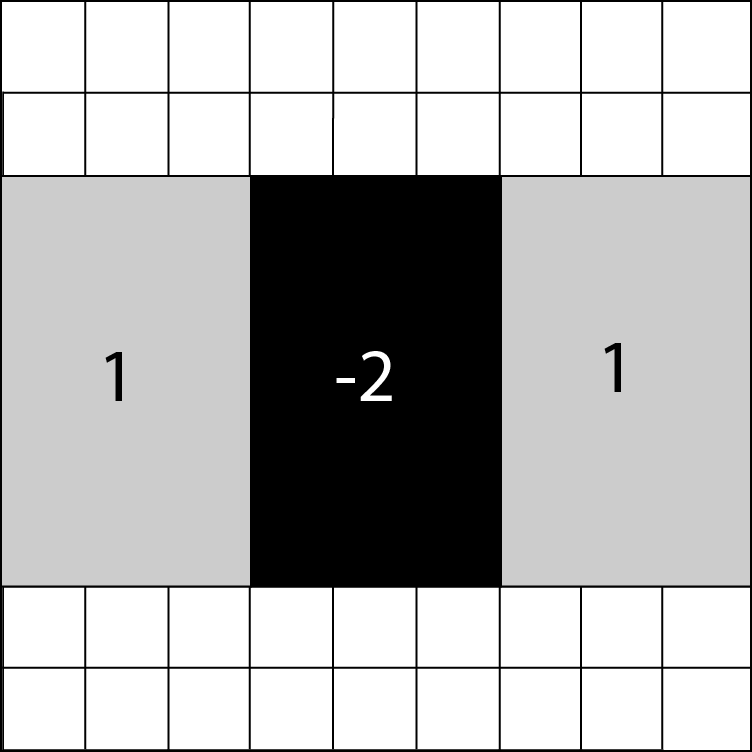
\includegraphics[width=\columnwidth]{figures/hessian/gaussian_second_order_kernel_xx}
		\caption{$\frac{\partial^2 G}{\partial x_1^2}$}
	\end{subfigure}
	\begin{subfigure}[b]{0.3\columnwidth}
		\centering
		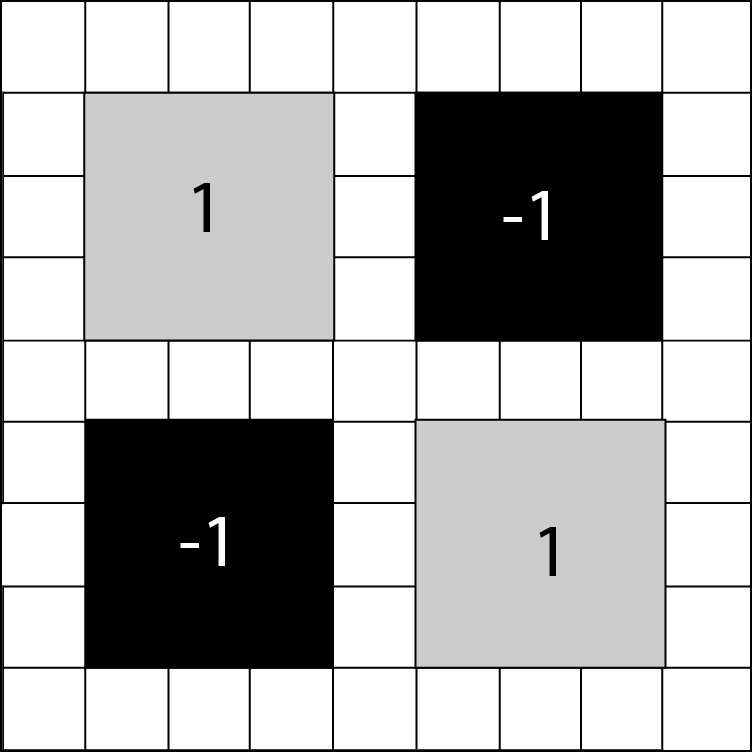
\includegraphics[width=\columnwidth]{figures/hessian/gaussian_second_order_kernel_xy}
		\caption{$\frac{\partial^2 G}{\partial x_1 x_2}$}
	\end{subfigure}
	\begin{subfigure}[b]{0.3\columnwidth}
		\centering
		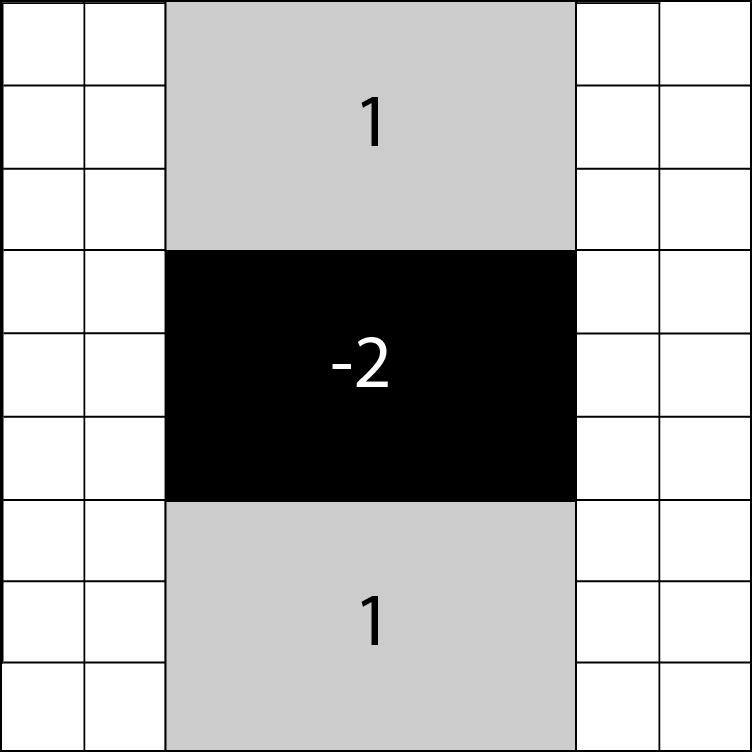
\includegraphics[width=\columnwidth]{figures/hessian/gaussian_second_order_kernel_yy}
		\caption{$\frac{\partial^2 G}{\partial x_2^2}$}
	\end{subfigure}
	\caption{$9 \times 9$ discrete approximations of the Gaussian second order derivative with $\sigma=1.2$}
	\label{fig_gaussian_kernels}
\end{figure}

Another speed optimization presented in SURF takes advantage of the form of the discrete kernels. Since the approximated kernels are composed of rectangles of constant value, they can be decomposed into a set of box filters. Box filters can be computed quickly with the use of integral images. The general form of the integral image of an $M \times N$ image $I$ is shown in Equation \ref{eq_integral_image}.

\begin{equation}
\int I = \begin{bmatrix}
I(0,0) & \sum\limits_{m=0}^1 I(0,m) & \cdots & \sum\limits_{m=0}^M I(0,m) \\
\sum\limits_{n=0}^1 I(n,0) & \sum\limits_{n=0}^1 \sum\limits_{m=0}^1 I(n,m) & & \vdots \\
\vdots & & \ddots & \vdots \\
\sum\limits_{n=0}^N I(n,0) & \cdots & \cdots & \sum\limits_{n=0}^N \sum\limits_{m=0}^M I(n,m)
\end{bmatrix}
\label{eq_integral_image}
\end{equation}

Integral images decrease the computational complexity of finding the sum of an area in the input image. The computational complexity of strict kernel convolution at a point scales with the size of the kernel and is of the order $O(N^2)$ where the kernel is $N \times N$. A box filter can be decomposed into finding the sum of an area in the image and scaling it. Finding the sum from the integral image can be performed in $O(1)$ as shown in Equation \ref{eq_integral_image_box}. 

\begin{equation}
\sum\limits_{n=w}^y \sum\limits_{m=x}^z = \int I(y,z) - \int I(w-1,z) - \int I(y,x-1) + \int I(w-1, x-1)
\label{eq_integral_image_box}
\end{equation}

This makes the computation of the Hessian matrix scale only in terms of the image size, yielding no additional penalty for operating on different scale spaces.

\subsubsection{SURF Implementations for FPGA Devices}

The relatively low computational complexity makes SURF a popular choice for FPGA applications. Battezzati et al. present an architecture using accumulators for computing the integral image pipelined through the Hessian computation and storing detected feature points in a first in, first out (FIFO) cache \cite{battezzati_surf_2012}. These are matched against a stored set of feature points. Chen et al. present improvements on this approach by parallelizing the computation of different scale spaces \cite{chen_fpga-based_2016}. The implementation in this thesis follows these approaches with some additional improvements for speed based on the use case of matching against another image rather than a stored set of features.

\subsection{Iterative Closest Point Algorithm}

The crucial step in aligning the two images is the computation of an affine transform mapping one image into the space of the other. Once the images are aligned, they can be fused. A combination of SURF and the iterative closest point algorithm are used to compute this transform. Iterative closest point was designed as a method for aligning 3-D point cloud data \cite{chen_object_1992}. In its simplest form, the algorithm follows the following steps:

\begin{enumerate}
	\item Each point in the set of points to be transformed is matched against the closest (usually Euclidean distance) point in the reference set of points.
	\item A transformation is estimated to minimize the distance between the transform set and their matches in the reference set of points.
	\item The transform is applied to the points.
\end{enumerate}

This process is repeated, converging to the local minimum that is the match between the two point sets.

Let $X_r(i)$ be the $i^{th}$ point in the set of reference points onto which the transform points, $X(j)$, where $j$ is the index of the closest point to $X_r(i)$ in $X$, will be projected. The general form for this transformation $M$ is shown in Equation \ref{eq_general_icp_mapping}, and the expanded matrix form can be seen in Equation \ref{eq_expanded_icp_mapping}. In the expanded matrix form $M$ is decomposed into $R$, a $2 \times 2$ rotation matrix, and $T$, a translation offset.

\begin{equation}
X_r(i) = X(j) \cdot M
\label{eq_general_icp_mapping}
\end{equation}

\begin{equation}
\begin{bmatrix}
X_r(i)_1 \\
X_r(i)_2 \\
1 
\end{bmatrix}
=
\begin{bmatrix}
X(j)_1 & X(j)_2 & 1
\end{bmatrix}
\cdot
\begin{bmatrix}
R_{11} & R_{12} & T_1 \\
R_{21} & R_{22} & T_2 \\
0 & 0 & 1
\end{bmatrix}
\label{eq_expanded_icp_mapping}
\end{equation}

This equation only solves for $M$ for a single point relation, but can be restructured to contain
the whole set of $N$ points as shown in Equation \ref{eq_full_icp_matrix}. In this equation $P$ is a function $P: i \rightarrow j$ mapping the closest points in each set.

\begin{equation}
\resizebox{\columnwidth}{!} {$
\begin{bmatrix}
X_r(0)_1 \\
X_r(0)_2 \\
X_r(1)_1 \\
X_r(1)_2 \\
\vdots \\
X_r(N-1)_1 \\
X_r(N-1)_2
\end{bmatrix}
=
\begin{bmatrix}
X(P(0))_1 & X(P(0))_2 & 1 & 0 & 0 & 0 \\
0 & 0 & 0 & X(P(0))_1 & X(P(0))_2 & 1 \\
X(P(1))_1 & X(P(1))_2 & 1 & 0 & 0 & 0 \\
0 & 0 & 0 & X(P(1))_1 & X(P(1))_2 & 1 \\
\vdots & & & & & \vdots \\
X(P(N))_1 & X(P(N))_2 & 1 & 0 & 0 & 0 \\
0 & 0 & 0 & X(P(N))_1 & X(P(N))_2 & 1 
\end{bmatrix}
\cdot
\begin{bmatrix}
R_{11} \\
R_{12} \\
T_1 \\
R_{21} \\
R_{22} \\
T_2
\end{bmatrix}
$}
\label{eq_full_icp_matrix}
\end{equation}

Solving for $M$ in this way maps all points in $X$ to their closest points in $X_r$ based on an orthogonal projection with the error minimized in a least-square sense. 

In this form, the transform $M$ will include shear transformations and non-uniform scaling. The computation can be simplified by forcing the second basis vector in $R$ to be orthogonal to the first. The two cameras are expected to be be physically in the same plane, and as such, non-uniform scaling and shear transformations are not expected for alignment. By setting $R_{21} = -R_{12}$ and $R_{22} = R{11}$, the computation of $M$ can be reduced as shown in Equation \ref{eq_reduced_icp_matrix}.

\begin{equation}
\begin{bmatrix}
X_r(0)_1 \\
X_r(0)_2 \\
X_r(1)_1 \\
X_r(1)_2 \\
\vdots \\
X_r(N-1)_1 \\
X_r(N-1)_2
\end{bmatrix}
=
\begin{bmatrix}
X(P(0))_1 & X(P(0))_2 & 1 & 0 \\
X(P(0))_2 & -X(P(0))_1 & 0 & 1 \\
X(P(1))_1 & X(P(1))_2 & 1 & 0 \\
X(P(1))_2 & -X(P(1))_1 & 0 & 1 \\
\vdots & & & \vdots \\
X(P(N-1))_1 & X(P(N-1))_2 & 1 & 0 \\
X(P(N-1))_2 & -X(P(N-1))_1 & 0 & 1 \\
\end{bmatrix}
\cdot
\begin{bmatrix}
R_{11} \\
R_{12} \\
T_1 \\
T_2
\end{bmatrix}
\label{eq_reduced_icp_matrix}
\end{equation}

If scaling is disallowed, and the transformation consists of only a translation and a rotation, this can be reduced further. Consider first computing the centroids of the point sets as in Equation \ref{eq_centroid}.

\begin{equation}
C = \frac{1}{N}\sum\limits_{i=0}^{N-1}X(i)
\label{eq_centroid}
\end{equation}

Based on the closest point matching, the covariance matrix $H$ can be computed as in Equation \ref{eq_covariance}.

\begin{equation}
H=\sum\limits_{i=0}^{N-1} (X(P(i)) - C) \cdot (X_r(i) - C_r)^T
\label{eq_covariance}
\end{equation}

The singular value decomposition $U\Sigma V = SVD(H)$ can be used to compute the rotation $R=VU^T$, where the translation is the distance between the centroids.

The performance of iterative closest point can be further improved by making it more sensitive to errors. Chetverikov introduced a variant of iterative closest point referred to as trimmed iterative closest point (TrICP) \cite{chetverikov_trimmed_2002}. TrICP is more robust to errors by eliminating points that introduce error into the matching. Some detected features points will not have correspondences between images. By eliminating these points, the overall error can be reduced to compute a more accurate transform.

\subsection{Singular Value Decomposition (SVD)}

Let Equation \ref{eq_reduced_icp_matrix} be of the form $X=Q \cdot M$. In order to compute the transform $M$, the equation must be restructured as in Equation \ref{eq_svd_inverse}.

\begin{equation}
Q^{-1} X = M
\label{eq_svd_inverse}
\end{equation}

$Q$ is not a square matrix, and as such is not invertible, but its pseudoinverse can be used in this instance. The pseudoinverse is computed through the use of singular value decomposition. The use of singular value decomposition to compute the transform is the source of the least squares fitting achieved by iterative closest point.

This is necessary for computing transforms with more degrees of freedom, however for rigid body transformations, it is sufficient to find the singular value decomposition of the covariance matrix $H$, a $2 \times 2$ matrix for which a closed form solution does exist\cite{blinn_consider_1996} and is shown in Equation \ref{eq_svd_decomp}.

\begin{equation}
\resizebox{\columnwidth}{!} {$
\begin{gathered}
	\begin{bmatrix}
	A & B \\
	C & D
	\end{bmatrix}
	=
	\begin{bmatrix}
	cos\beta & sin\beta \\
	-sin\beta & cos\beta
	\end{bmatrix}
	\begin{bmatrix}
	w_1 & 0 \\
	0 & w_2
	\end{bmatrix}
	\begin{bmatrix}
	cos\gamma & sin\gamma \\
	-sin\gamma & cos\gamma
	\end{bmatrix}
	=
	\begin{bmatrix}
	E & H \\
	-H & E
	\end{bmatrix}
	+
	\begin{bmatrix}
	F & G \\
	G & -F
	\end{bmatrix}
	\\
	\frac{w_1 + w_2}{2} = \sqrt{E^2 + H^2}
	\\
	\frac{w_1 - w_2}{2} = \sqrt{F^2 + G^2}
	\\
	\gamma - \beta = tan^{-1}(G/F)
	\\
	\gamma + \beta = tan^{-1}(H/E)
\end{gathered}
$}
\label{eq_svd_decomp}
\end{equation}

\subsubsection{SVD Implementations for FPGA Devices}

Singular value decomposition can be performed on FPGAs by cascading a set of $2 \times 2$ cells \cite{wang_singular_2010}. Ledesma-Carillo et al. present a hardware efficient algorithm for computing singular value decompositions on large matrices using one-sided Jacobi rotations for computing SVD on arbitrary $M \times N$ matrices \cite{ledesma-carrillo_reconfigurable_2011}. One of these approaches is necessary if the sensor fusion must correct for scale or shear. It is worth noting that these approaches both require high utilization of the FPGA, and as such may be difficult to implement for large numbers of feature points.

In contrast, if only a rigid body transformation is required, then Equation \ref{eq_svd_decomp} can be implemented trivially using CORDIC approximations for the square root and arctangent functions.


\subsection{Laplacian Fusion}

Laplacian pyramids of images have their origin as a strategy for image encoding \cite{burt_laplacian_1983}. A Gaussian blur is applied to the image, and the image is downsampled to half of its original size. At each level above the lowest level of the Gaussian pyramid, the level below is upsampled to match the scale of the current level. The difference between the upsampled image and the current scale level image is the Laplacian of the image. At a single level, the Laplacian can be thought of as the error introduced by applying a Gaussian and Box filter.

The property of the Laplacian that makes it ideal for fusion is its ability to capture the high frequency components in an image through the use of simple kernel operators that are easily implemented in hardware. The difference between a blurred image and the original will have higher magnitude in the areas where the image was sharpest.

The fusion of two images can be thought of as a function of the two images $X$ and $Y$ of dimension $M \times N$ where $Z = f(X, Y)$, a single image of dimension $M \times N$. A naive approach to fusion would be to compute the Laplacians and use their magnitudes to select a pixel from either $X$ or $Y$ as shown in Equation \ref{eq_naive_fusion}. In this context, $|L(x)|$ represents the absolute value of the Laplacian of the input.

\begin{equation}
Z(i,j)=
\begin{cases}
X(i,j) & |L(X(i,j))| \ge |L(Y(i,j))| \\
Y(i,j) & otherwise
\end{cases}
\label{eq_naive_fusion}
\end{equation}

This approach does not account for variations in colorspace between the two images. More saturated images would likely have a higher valued Laplacian simply because it is brighter, therefore having higher magnitudes at individual pixels. This approach also will not facilitate smooth stitching of the images. Contiguous regions of selection from one image will be adjacent to regions from the other with no transition, producing a grainy effect at areas of high frequency.

A more correct approach would involve using the Laplacian in a weighted sum to combine the pixels of the images, rather than simply selecting them, as shown in Equation \ref{eq_weighted_fusion}.

\begin{equation}
\resizebox{\columnwidth}{!} {$
	Z(i,j) = \frac{|L(X(i,j))|}{|L(X(i,j))| + |L(Y(i,j))|} \cdot X(i,j) + \frac{|L(Y(i,j))|}{|L(X(i,j))| + |L(Y(i,j))|} \cdot Y(i,j)
	\label{eq_weighted_fusion}
	$}
\end{equation}

\section{Proposed Method}

The implementation of this design was performed on a ZedBoard Zynq-7000 ARM/FPGA SoC Development Board.

\subsection{Camera Interface}

The design was implemented using a pair of OV7670 VGA cameras. These cameras feature an $I^2C$ interface for configuration, and generate hsync and vsync VGA timing signals along with 8 bits of data. They can be configured to output 16-bit RGB(565) with half of the RGB signal sent on each clock pulse. Configured this way, the camera outputs a resolution of $640$ by $480$ pixels at $30Hz$. 

\subsection{Streaming Kernel Operators}

Performing kernel convolution in real time is complicated by the fact that a pixel has data dependencies on its neighbors. As such, the input data must be buffered until all of the necessary data is available to perform convolution at a given point. The buffer size must be at least $N \times W + M$ where the kernel is $M \times N$ and the image is of width $W$. On FPGAs, this minimally sized buffer can be implemented using LUTRAM which also has the advantage of being able to act as a set of shift registers. The convolution multipliers and adders can be attached to a single set of cells, and the data can be shifted through the array as it streams. The architecture for this scan chain approach for computing $3 \times 3$ kernel convolution can be seen in Figure \ref{fig_block_scanchain}.

\begin{figure}[h]
	\centering
	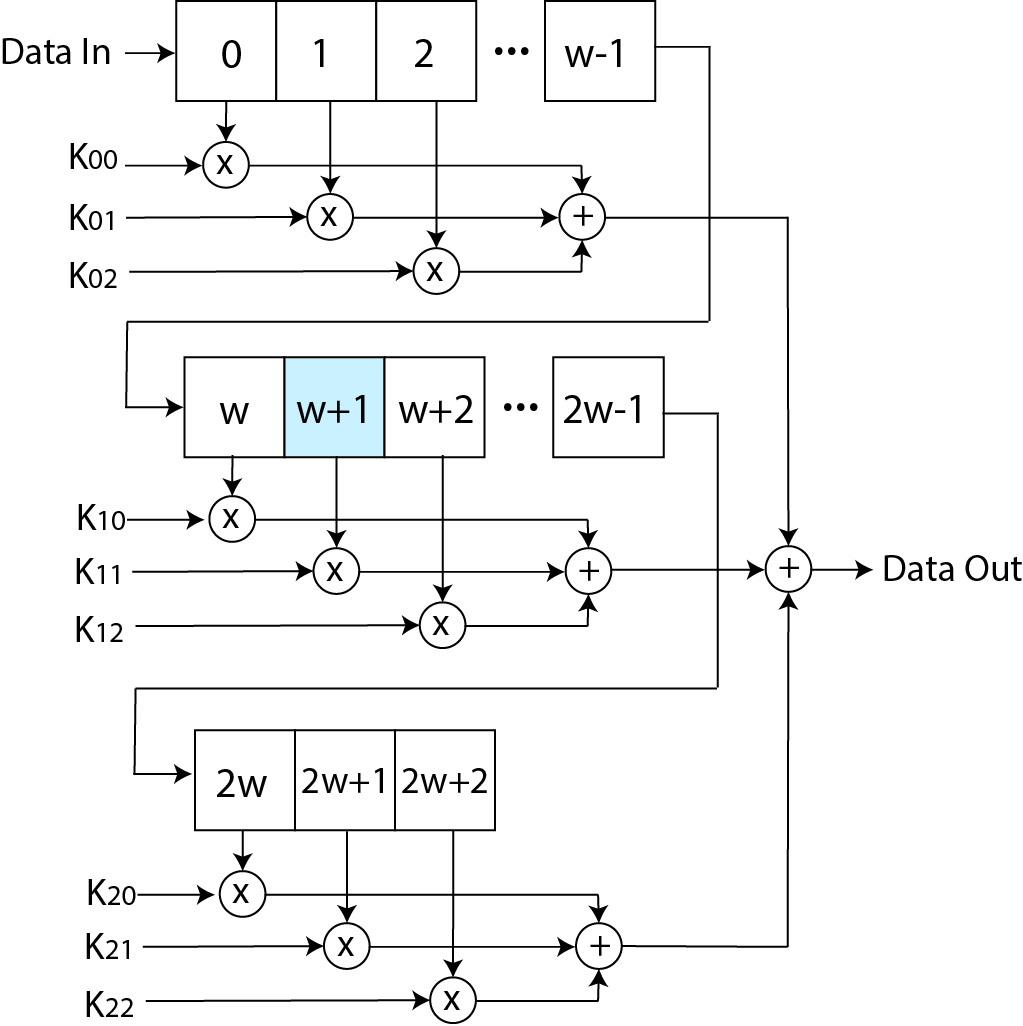
\includegraphics[width=0.9\columnwidth]{figures/block/scanchain}
	\caption{Block diagram for computing $3 \times 3$ kernel convolution on a data stream using a scan chain}
	\label{fig_block_scanchain}
\end{figure}

This scan chain approach to kernel convolution is a fast and utilization efficient approach to performing kernel convolution on streamed data. However, LUTRAM on most FPGAs is a limited resource, and as such, large kernels and image widths will make it difficult to implement a design. Implementing an LUTRAM scan chain for performing operations on $9 \times 9$ kernels with an image width of $640$ pixels on the chipset used for this design consumed $96\%$ of the available LUTRAM. Since it was necessary to implement two hessian operators, one for each camera, an approach was devised to utilize the slower, but more plentiful block RAM.

\subsubsection{Hessian Kernel Operators}

The kernels discussed in this section are the $9 \times 9$ discrete approximations shown in Figure \ref{fig_gaussian_kernels}. If straightforward kernel convolution were to be implemented, it would require sampling all points with non-zero kernel values which would not be realistic for performing these operators in real time. Instead, the integral image is used to reduce the number of required sampling points. Recall that the integral image can be used to compute the area in a rectangle by sampling the corners, adding the bottom-right corner and top-left corner, and subtracting the bottom-left corner and top-right corner. As such, the required sampling points for the SURF kernels are highlighted in Figure \ref{fig_gaussian_integral_kernels}.

\begin{figure}[h]
	\centering
	\begin{subfigure}[b]{0.3\columnwidth}
		\centering
		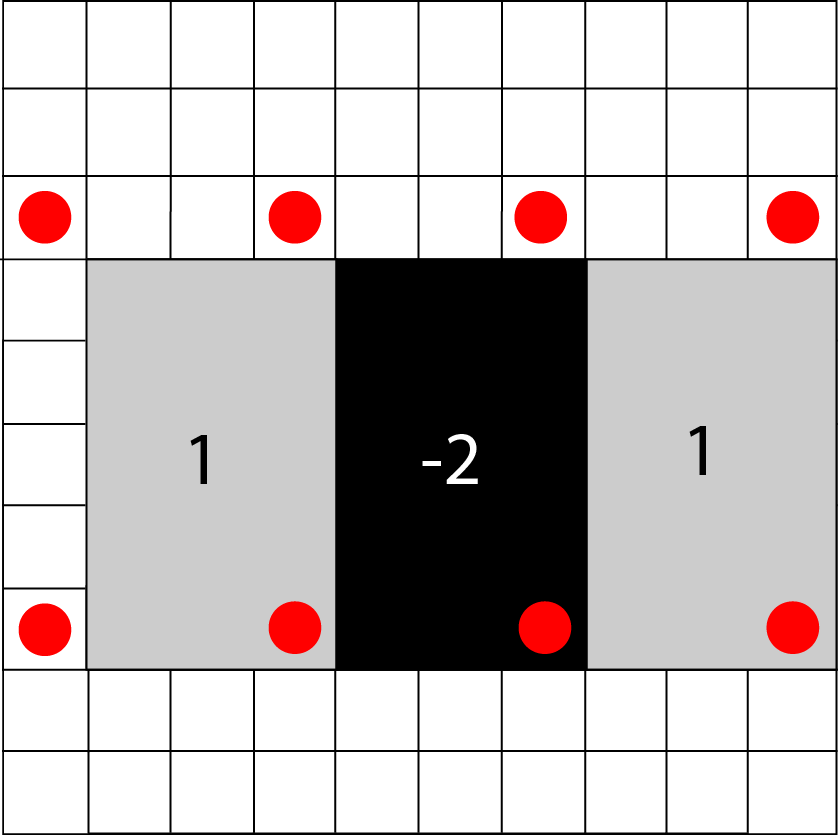
\includegraphics[width=\columnwidth]{figures/hessian/gaussian_second_order_kernel_xx_integral}
		\caption{$\frac{\partial^2 G}{\partial x_1^2}$}
	\end{subfigure}
	\begin{subfigure}[b]{0.3\columnwidth}
		\centering
		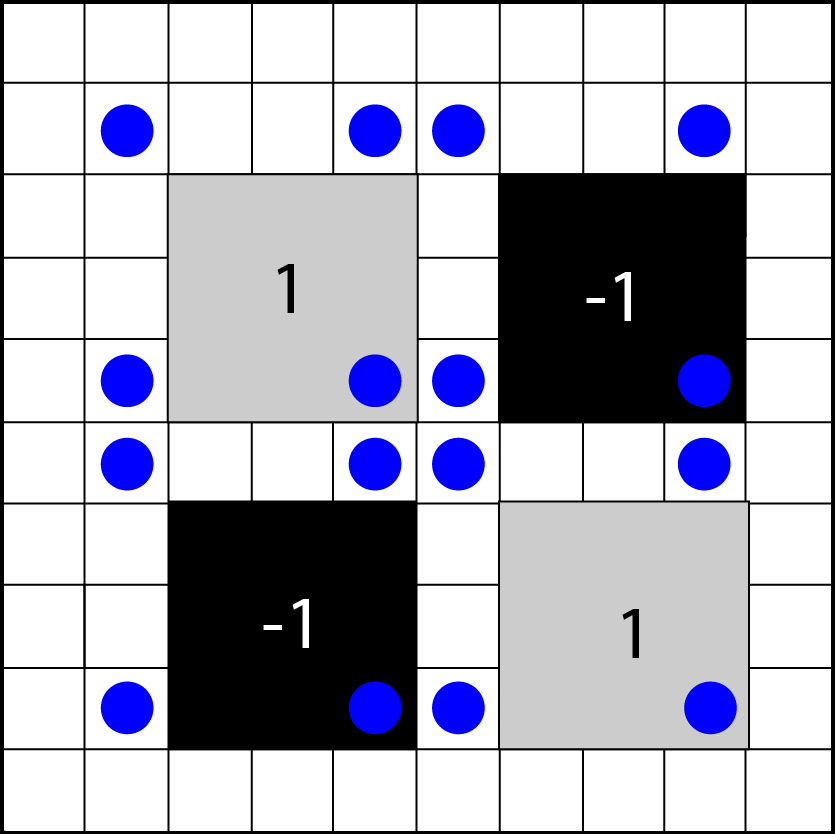
\includegraphics[width=\columnwidth]{figures/hessian/gaussian_second_order_kernel_xy_integral}
		\caption{$\frac{\partial^2 G}{\partial x_1 x_2}$}
	\end{subfigure}
	\begin{subfigure}[b]{0.3\columnwidth}
		\centering
		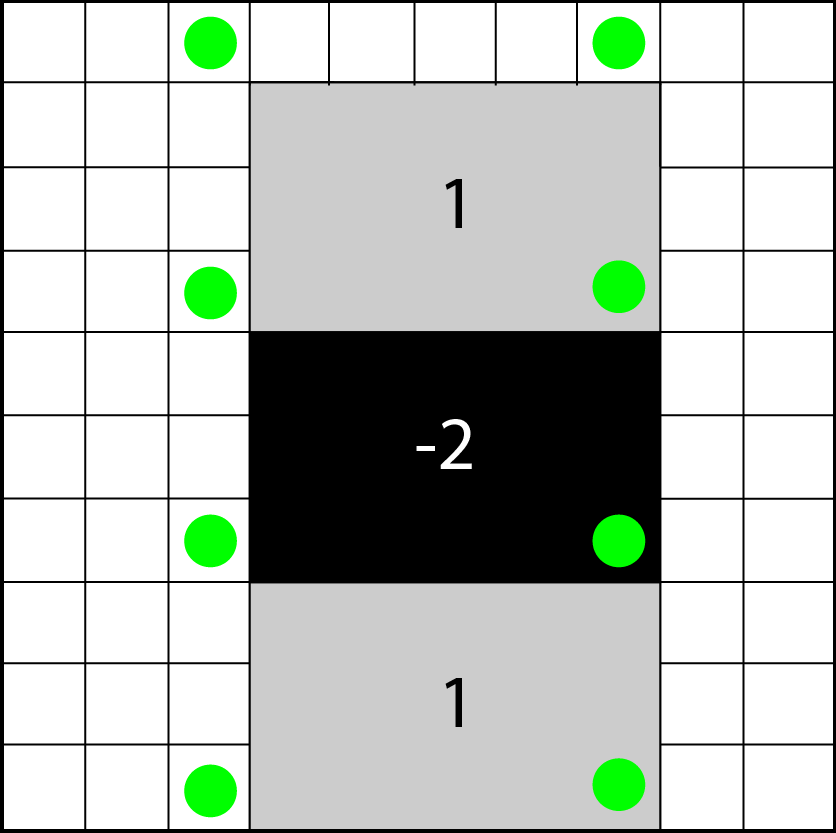
\includegraphics[width=\columnwidth]{figures/hessian/gaussian_second_order_kernel_yy_integral}
		\caption{$\frac{\partial^2 G}{\partial x_2^2}$}
	\end{subfigure}
	\caption{$9 \times 9$ SURF kernels with marked integral sampling points}
	\label{fig_gaussian_integral_kernels}
\end{figure}

It can be observed in Figure \ref{fig_gaussian_integral_kernels} that the worst-case for the data dependencies is the bottom-right point in $\frac{\partial^2 G}{\partial x_2^2}$. If the Hessian determinant is to be computed with minimal latency, it should be computed when that point becomes available. In order to compute the integral at a point, the integral above, to the left, and to the top-left of the desired point must be sampled. From this, it can be concluded that thirty-four points must be sampled to compute the Hessian determinant (eight from $\frac{\partial^2 G}{\partial x_1^2}$, sixteen from $\frac{\partial^2 G}{\partial x_1 x_2}$, seven from $\frac{\partial^2 G}{\partial x_2^2}$, and three to compute the integral). 

In order to do this in real time, the Hessian determinant must be computable within a pixel clock cycle. Given a resolution of $640$ by $480$ at $30$ frames per second, this is a pixel clock speed of $12.5 MHz$. In this implementation, block RAM has a latency of three clock cycles. In order to compute the determinant in a single pixel clock cycle, the Hessian block is clocked at $200 MHz$, giving it $16$ clock cycles for every pixel clock cycle. A $200 MHz$ clock has a period of only $5ns$ which makes pipelining of instructions important in order to meet timing. A dual port block RAM was used, with addressing using the lower bits of $y$ to map into a modular address space of $16$ rows. The dual port RAM effectively allows for $32$ read/write operations within the pixel clock period. An LUTRAM cache containing the integral values for the last row up to the top-left point required for the integral image reduces the number of memory reads for required points to $29$, along with a single memory write to place the last value in the cache into the block RAM. 

The process is pipelined by splitting up the determinant computation into small operations that execute as the data becomes available from the block RAM. It is worth noting that this implementation does not need to be modified to compute Hessian determinants in different scale spaces. Larger kernels still have the same number of points that must be sampled, but the required block RAM for the design does grow with the kernel size.

\subsubsection{Average Filter Approximation of Single Level Laplacian Pyramid}

In this design, only a single level of the Laplacian pyramid is used for fusion. In a single level, a Gaussian blur is applied to the image. It is downsampled, upsampled, and subtracted from the original. The downsampling and upsampling in a single level can be approximated as an average filter without performing the costly operation of modifying the resolution of the image. In this design, the Gaussian and average filters were implemented as a set of scan chains to perform $3 \times 3$ kernel convolution.

\subsubsection{Application of Non-maximum Suppression}

Though not a kernel operator, non-maximum suppression depends on the data points around it. Non-maximum suppression is to be applied to the Hessian determinant values in order to reduce them to a smaller, more precise set of features. In a $3 \times 3$ neighborhood, if the central pixel is not the maximum, it is set to zero. In this way, only the peak features remain for processing. The $3 \times 3$ neighborhood search was implemented as a $3 \times 3$ scan chain with comparison operators.

\subsection{Computation of Transform from Detected Features}

As features are generated, they are passed into a feature buffer as a tuple of their magnitude, x, and y coordinates. The buffer is made up of bubble-sort cells as shown in Figure \ref{fig_bubblesort}.

\begin{figure}[h]
	\centering
	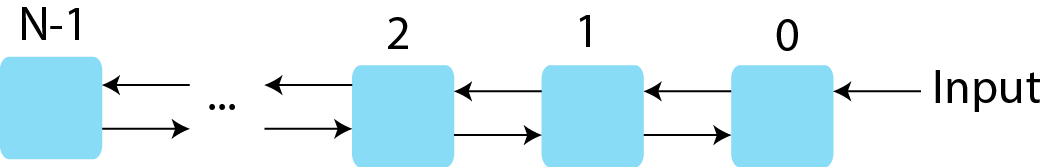
\includegraphics[width=\columnwidth]{figures/block/bubblesort}
	\caption{Bubble-sort architecture of the feature buffer}
	\label{fig_bubblesort}
\end{figure}

On the rising edge of the clock, the even cells swap values with their neighbor to the left if the cell contains a greater value than its neighbor. On the falling edge, the odd cells do the same. In this way, the highest valued elements propagate to the top of the buffer, and lower valued elements are dropped out of the bottom. The comparison criteria for this operation is the Hessian magnitude, and the sort is active for as long as features are being generated. At the end of the frame, the buffer contains only the points with the highest Hessian magnitudes.

Once the points have been collected, the transform set is compared to the reference set and correspondences are assigned based on euclidean distance to find the closest point. This is done via a brute-force search. Every point is compared to every other, and the closest one emerges. 

For low numbers of feature points, the inefficiency of brute-force search is mitigated by its simplicity. In hardware, a brute force comparison like this does not suffer from additional time complexity since the comparisons all happen in parallel. However, the space complexity and fanout of the circuit goes up exponentially as more cells are added.

This architecture is only useful for small numbers of feature points. The high fanout of the brute force comparison quickly becomes unmanageable to route in most designs with more than a handful of features. In the case that this becomes difficult, it is possible to trade the space complexity of the design for time complexity by making the computation iterative.

In this approach, a match register holds the point that is the current closest match. A point from the reference set is loaded into a register, A. Then, each point in the transform set is loaded into a register, B, in turn. If the distance between the loaded value and the value in register A is less than the distance between the value stored in the match register and register A, then the loaded value from register B is placed into the match register. This is repeated for all elements in the reference set to find their closest points in the transform set.

\subsection{Application of Transform to Real-Time Data}

The reference image remains fixed and is outputted as normal. The address for the transform image is decomposed into x and y coordinates. This is multiplied through the computed transform, and the transformed coordinates are used to select pixels from the frame buffer. The reference pixel and transform pixel are then fused together to create the output stream.

The transform is recomputed at the end of the frame from the detected features and then applied to the next generation of incoming data. In this way, the transform is additively refined as in iterative closest point. The transform computed for a frame is concatenated with the transform from the last frame, eventually converging to a local error minimum for alignment in a least squares sense. 

\section{Conclusions}
The proposed pipeline architecture for computing the Hessian determinants with minimal latency allows FPGA implementation of video alignment where the video sources fields of view varies with time. The technique has potential for future use in video stabilization where consecutive video frame fields of view vary due to camera jitters. The treatment of each frame as a generation of feature points to be transformed to a local error minimum as opposed to a more rigid architecture of performing multiple iterations on one feature set helps alleviate the overhead of the design, and make it realizable. The available chipset was not of sufficient size to perform the larger corrections of scale and shear due to the prohibitive nature of the instantiating large arrays of SVD solving cells. However, on a more robust chipset, scale and shear should also be correctable factors, as well as giving the ability to compute the transform from a larger set of feature points.

\bibliographystyle{plain}
\bibliography{thesis}

\end{document}
